\documentclass[12pt,aspectratio=169]{beamer}
\input{header_beamer}
\usetheme{Boadilla}
\usecolortheme{beaver}
\setbeamertemplate{page number in head/foot}{}
\setbeamertemplate{navigation symbols}{}
\title{Lecture-27: Poisson process on the half-line}
\date{}

\begin{document}
\pagestyle{empty}
\maketitle

\begin{frame}{Simple point processes on the half-line} 
A stochastic process defined on the half-line $N: \Omega \to \Z_+^{\R_+}$ is a \textbf{counting process} if
\begin{enumerate}
  \item $N_0 = 0$, and 
  \item for each $\omega \in \Omega$, the sample path $N(\omega): \R_+ \to \Z_+$ is non-decreasing, integer valued, and right continuous function of time $t \in \R_+$.% and at points of discontinuity $(N_t- N(t^{-}))\le 1,~~\forall \omega \in \Omega$. 
\end{enumerate}
\end{frame}

\begin{frame}
%Each discontinuity of the sample path of the counting process can be thought of as a jump of the process, as shown in the figure below.  
%A simple counting process has unit jump size almost surely.  
%General point processes in higher dimensions do not have an inter-arrival time interpretation. 

\begin{center}
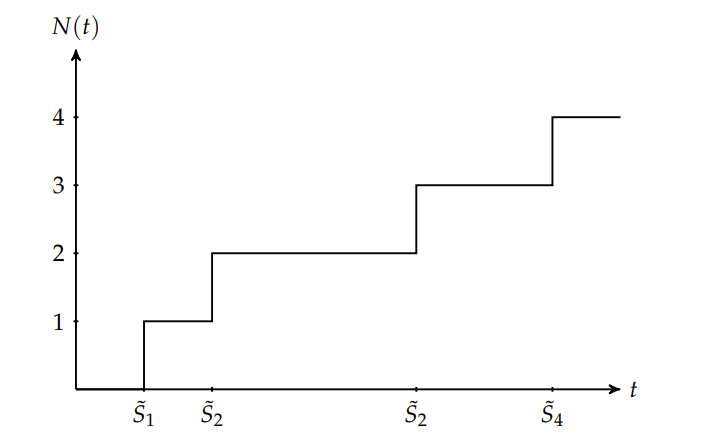
\includegraphics[width=0.8\linewidth]{Figures/Poisson_counting_process.png}
\captionof{figure}{Sample path of a simple counting process.}
\label{Fig:Poisson}
\end{center}
\end{frame}


\begin{frame}
\begin{Definition} 
The points of discontinuity are also called the \textbf{arrival instants} of the counting process $N$. 
The \textbf{$n$th arrival instant} is a random variable denoted $\tS_n: \Omega \to \R_+$, 
defined inductively as 
\meq{2}{
&\tS_0 \triangleq 0, &&\tS_n \triangleq \inf\set{t \ge 0: N_t \ge n},\quad n \in \N.
}
\end{Definition}
\begin{Definition}<2->
The \textbf{inter arrival time} between $(n-1)${th} and $n${th} arrival is denoted by $X_n$ and written as
$X_n \triangleq \tS_n - \tS_{n-1}$. 
\end{Definition}
\end{frame}

\begin{frame}
\begin{block}{Reminder} 
For a simple point process, we have
$P\set{X_{n} = 0} = P\set{X_n\le 0} = 0.$
\end{block}
\begin{block}{Lemma}<2-> 
Simple counting process $N:\Omega\to\Z_+^{\R_+}$ and arrival process $\tS:\Omega\to\R_+^\N$ are inverse processes, i.e. 
\EQ{
\set{\tS_n \le t} = \set{N_t \ge n}.
}
\end{block}
\begin{Proof}<3-> 
Let $\omega \in \set{\tS_n \le t}$, then $N_{\tS_n} = n$ by definition. 
Since $N$ is a non-decreasing process, we have $N_t \ge N_{\tS_n} = n$. 
Conversely, let $\omega \in \set{N_t \ge n}$, then it follows from definition that $\tS_n \le t$.
\end{Proof}
\end{frame}


\begin{frame}
\begin{cor} 
For arrival instants $\tS:\Omega\to\R_+^\N$ associated with a counting process $N:\Omega\to\Z_+^{\R_+}$ 
we have 
$
\set{\tS_n \le t, \tS_{n+1} > t} = \set{N_t = n} 
$
for all $n \in \Z_+$ and $t \in \R_+$. 
\end{cor}
\begin{Proof}<2->
It is easy to see that 
$\set{\tS_{n+1} > t } = \set{\tS_{n+1} \le t}^c = \set{N_t \ge n+1}^c = \set{N_t < n+1}$.
Hence, %the result follows by writing 
\EQ{
\set{N_t = n} = \set{N_t \ge n, N_t < n+1} = \set{\tS_n \le t, \tS_{n+1} > t}.
}
\end{Proof}
\end{frame}


\begin{frame}
\begin{block}{Lemma}
Let $F_n(x)$ be the distribution function for $S_n$, then 
$P_n(t) \triangleq P\set{N_t = n} = F_{n}(t)-F_{n+1}(t)$. 
\end{block}

\begin{Proof}<2->
It suffices to observe that following is a union of disjoint events,
\EQ{
\set{\tS_n \le t } = \set{\tS_n \le t, \tS_{n+1} > t} \cup \set{\tS_{n} \le t, \tS_{n+1} \le t}.
}
\end{Proof}
\end{frame}





\begin{frame}{IID exponential inter-arrival times characterization}

\begin{prop} 
The counting process $N:\Omega\to\Z_+^{\R_+}$ 
associated with a simple Poisson point process $S:\Omega\to\R_+^\N$ 
is Markov. 
\end{prop}
\end{frame}

\begin{frame}
\begin{Proof} 
We define the event space $\sF_t \triangleq \sigma(N_s: s \le t)$ as the history of the process until time $t \in \R_+$. 
Then, from the independent increment property of Poisson processes, we have for any historical event $H_s \in \sF_s$ 
\eq{
P(\set{N_t = n}\given H_s\cap\set{N_s = k})
&= P(\set{N_t-N_s = n-k} \given H_s\cap \set{N_s = k}) \\
&= P(\set{N_t = n}\given \set{N_s = k}). 
}
The transition probability matrix is $P(s,t)$ with its $(k,n)$th entry given by $e^{-\Lambda(s,t]}\frac{(\Lambda(s,t])^{n-k}}{(n-k)!}$. 
\end{Proof}
\end{frame}


\begin{frame}
\begin{block}{Reminder}
A Markov process $X:\Omega\to\sX^\R$ is time homogeneous if the transition matrix $P(s,t) = P(t-s)$ for all $t \ge s$. 
Thus the counting process for a homogeneous Poisson point process is time homogeneous Markov process, as the transition probability matrix $P(s,t) = P(t-s)$ with its $(k,n)$th entry given by $e^{-\lambda(t-s)}\frac{(\lambda(t-s))^{n-k}}{(n-k)!}$. 
\end{block}
\begin{block}{Theorem}<2->
The counting process $N:\Omega\to\Z_+^{\R_+}$ 
associated with a simple Poisson point process $S:\Omega\to\R_+^\N$ 
is strongly Markov. 
\end{block}
\end{frame}


\begin{frame}
\begin{prop}
A simple counting process $N:\Omega\to\Z_+^{\R_+}$ is associated with a \textbf{homogeneous Poisson process} with a constant intensity density $\lambda$, 
iff the inter-arrival time sequence $X:\Omega\to\R_+^\N$ are \iid random variables with an exponential distribution of rate $\lambda$. 
\end{prop}
\begin{block}{Proof}<2->
Let $N_t$ be a counting process associated with a homogeneous Poisson point process on half-line with constant intensity density $\lambda$. 
From equivalence $iii\_$ in the Theorem on Equivalences, we obtain for any positive integer $t$, 
\EQ{
P\set{X_1 > t} = P\set{N_t = 0} = e^{-\lambda t}. 
}
\end{block}
\end{frame}

\begin{frame}
\begin{block}{Proof}
It suffices to show that inter-arrivals time sequence $X:\Omega\to\R_+^\N$ is \iid.  
We can show that $N$ is Markov process with strong Markov property. 
Since the sequence of ordered points $\tS:\Omega\to\R_+^\N$ is a sequence of stopping times for the counting process, 
it follows from the strong Markov property of this process that $(N_{\tS_n+t} - N_{\tS_n}: t \ge 0)$ is independent of $\sigma(N_s: s \le \tS_n)$ and hence of $\tS_n$ and $N_{\tS_n}$. 
Further, we see that
\EQ{
X_{n+1} = \inf\set{t > 0: N_{\tS_n+t} - N_{\tS_n}  = 1}. 
}
It follows that $X:\Omega\to\R_+^\N$ is an independent sequence. 
For homogeneous Poisson point process, we have $N_{\tS_n+t}-N_{\tS_n} = N_t$ in distribution, 
and hence $X_{n+1}$ has same distribution as $X_1$ for each $n \in \N$. 
\end{block}
\end{frame}

\begin{frame}
\begin{Proof}[Proof continued]
For the given \iid inter-arrival time sequence $X:\Omega\to\R_+^\N$ distributed exponentially with rate $\lambda$, we define the $n$th arrival instant $\tS_n \triangleq \sum_{i=1}^nX_i$ for each $n \in \N$, and the number of arrivals in time duration $(0,t]$ as $N_t\triangleq \sum_{n\in\N}\SetIn{\tS_n\le t}$ for all $t\in \R_+$. 
It follows that $N_t$ is path wise non-decreasing, integer-valued, right continuous, and simple since $P\set{X_1 \le 0} = 0$. 
Therefore, $N$ is a simple counting process such that 
\EQ{
P\set{N_t = 0} = P\set{X_1 > t} = e^{-\lambda t}. 
}
It follows that the void probabilities are exponential and hence the random variable $N_t$ is Poisson with parameter $\lambda t$ for all $t \in \R_+$. 
Hence, $N$ is a counting process associated with a homogeneous Poisson process with the constant intensity density $\lambda$ from the equivalence $ii\_$ in Theorem on Equivalences. 
\end{Proof}
\end{frame}


\begin{frame}
For many proofs regarding Poisson processes, 
we partition the sample space with the disjoint events $\set{N_t = n}$ for $n \in \Z_+$. 
We need the following lemma that enables us to do that. 
\begin{block}{Lemma}<2->
For any finite time $t > 0$, the number of points on the interval $(0,t]$ from a Poisson process is finite almost surely.
\end{block}

\begin{Proof}<3-> 
By strong law of large numbers, we have $\lim_{n \to \infty} \frac{S_{n}}{n} = \E[X_{1}] = \frac{1}{\lambda}$ almost surely. 
Fix $t > 0$ and we define a sample space subset $M = \set{\omega \in \Omega: N(\omega, t) = \infty }$. 
For any $\omega \in M$, we have $S_{n}(\omega)\le t$ for all $n \in \N$. 
This implies $\lim\sup_n\frac{S_{n}}{n} = 0$  and $\omega \not\in \set{\lim_n \frac{S_{n}}{n} = \frac{1}{\lambda} }$. 
Hence, the probability measure for set $M$ is zero. 
\end{Proof}
\end{frame}


\begin{frame}{Distribution functions}
\begin{block}{Lemma} 
The following are true for the $n$th arrival instant $\tS_n$ of the Poisson arrival process $\tS:\Omega\to\R_+^\N$ with constant intensity density $\lambda$.
\begin{enumerate}[(a)]
\item<2-> The moment generating function is 
$
M_{\tS_n}(\theta) = \E[e^{\theta \tS_n} ] = \frac{\lambda^n}{(\lambda-\theta)^n}\SetIn{\theta < \lambda} + \infty\SetIn{\theta \ge \lambda}.
$ 
\item<3-> The distribution function is  
$F_n(t) \triangleq P\set{\tS_n \le t} = 1 - e^{-\lambda t}\sum_{k=0}^{n-1}\frac{(\lambda t)^k}{k!}$.
\item<4-> The density function is Gamma distributed with parameters $n$ and $\lambda$. That is, $f_{n}(s) =\frac{\lambda (\lambda s)^{n-1}} {(n-1)!} e^{-\lambda s}$. 
\end{enumerate}
\end{block}
\end{frame}


\begin{frame}
\begin{cor} 
Consider the counting process $N:\Omega\to\Z_+^{\R_+}$ associated with the Poisson arrival process $\tS:\Omega\to\R_+^\N$ having constant intensity density $\lambda$. 
The following are true.
\begin{enumerate}[(a)]
\item<2-> The relation between distribution of $n$th arrival instant and probability mass function for the counting process is given by  $F_n(t)= \sum_{j \ge n}P_j(t)$. 
\item<3-> For each $t\in\R_+$, the probability mass function $P_{N_t}\in\cM(\Z_+)$ for discrete random variable $N_t:\Omega\to\Z_+$ is given by $P_n(t) \triangleq P_{N_t}(n) = P\set{N_t=n)}= e^{-\lambda t}\frac{(\lambda t)^{n}}{n!}$. 
\item<4->  The relation between distribution of $n$th arrival instant and the mean of the counting process is given by $\sum_{n \in \N}F_n(t) = \E N_t$. 
\item<5-> For each $t\in\R_+$, the mean  $\E[N_t] = \lambda t$, explaining the rate parameter $\lambda$ for the Poisson process. 
\end{enumerate}
\end{cor}
\end{frame}

\begin{frame}
\begin{Proof}
We observe the inverse relationship $\set{\tS_n \le t} = \set{N_t \ge n}$ for all $n \in \Z_+$ and $t\in\R_+$.  
\begin{enumerate}[(a)]
\item<2-> The result follows by taking the probability on both sides of the inverse relationship, to get  
$
F_n(t)  
= P\set{\tS_n \le t} 
= P\set{N_t \ge n}  
= \sum_{j \ge n}P\set{N_t = j}
= \sum_{j \ge n}P_j(t).
$
\item<3-> The result follows from the explicit from for the distribution of $\tS_n$ and recognizing that $P_n(t) = F_n(t) - F_{n+1}(t)$. 
\item<4-> The result from the following observation
$
\sum_{n \in \N}F_n(t) = \E\sum_{n \in \N}\SetIn{N_t \ge n} = \sum_{n \in \N}P\set{N_t \ge n} = \E N_t.
$
\item<5-> The result follows by summing the distribution function of the $n$th arrivals, to get 
$\E N_t = \sum_{n\in\N}F_n(t) = e^{-\lambda t}\sum_{n\in\N}\sum_{k \ge n}\frac{(\lambda t)^k}{k!} = 
\lambda t e^{-\lambda t}\sum_{k\in\N}\frac{(\lambda t)^{k-1}}{(k-1)!} = \lambda t$. 
\end{enumerate}
\end{Proof}
\end{frame}

\begin{frame}
\begin{block}{Reminder} 
A Poisson process is not a stationary process. 
That is, the finite dimensional distributions are not shift invariant. 
This is clear from looking at the first moment $\E N_t = \lambda t$, which is linearly increasing in time. 
\end{block}
\end{frame}
\end{document}
